%!TEX encoding = UTF-8 Unicode
% !TeX spellcheck = en_GB
%%%%%%%%%%%%%%%%%%%%%%%%%%%%%%%%%%%%%%
\chapter{ Associated $Zh$ production via gluon fusion at NLO }\label{chap:hz}
%%%%%%%%%%%%%%%%%%%%%%%%%%%%%%%%%%%%%%
%\section{Overview}
\par As we have seen in the previous sections, Higgs couplings to the weak vector bosons, i.e. $Z$ and $W$ is approaching the precision level. Moreover, the associated Higgs production with these bosons is the first channel used to observer the Higgs decaying into beauty quarks   $h \rightarrow b \bar{b}$ by both ATLAS and CMS~\cite{Aaboud:2018zhk, Sirunyan:2018kst}. Hence, the $ Vh$ Higgs production channel is one of the important channels to look for in the future runs of the LHC for better measurement of the $VVh$ coupling as well as Higgs coupling to the beauty quark. As the statistical and systematic uncertainties coming from the experimental setup of the LHC get reduced in the future runs, due to higher integrated luminosity and uprated detectors and analysis techniques. There is a  need to reduce theoretical uncertainties emerging from the perturbative calculations of  cross-sections. In order to achieve that, one should include more terms in the perturbative expansion in the couplings, particularly the string coupling $\alpha_s$. In this chapter, we are interested in the channel $pp\to Zh$, which is quark-initiated tree-level process at LO interpreted as \textbf{Drell-Yan process}~ \cite{Han:1991ia,Brein:2003wg}. This process has been computed up to next-to-next-to-leading-order (NNLO) in QCD ($\sim \alpha_s^2$), and
at next-to-leading-order (NLO) in the EW interactions ($\sim \alpha^2 $) \cite{Amoroso:2020lgh}.
%%
\par Despite arising for the first time at NNLO in perturbation theory to the partonic cross-section  , the gluon fusion channel $g g \rightarrow Zh$ has a non-negligible contribution to the hadronic cross-section of  $pp\to Zh$ process, which could reach $>16\%$ of the total cross-section contribution at $14$ TeV~\cite{Cepeda:2019klc}, see~\autoref{fig:hzratio} .The contribution becomes more significant when looking at large invariant mass bins in the differential cross-section. This is due to the significant abundance of gluons at the LHC for large $Q$ as well as the top quark initiated contribution near the $t\bar t$ threshold~\cite{Englert:2013vua}.  The gluon fusion channel has a higher scales uncertainties than the quark induced one, and due to the significant contribution of the former, and the absence of gluon fusion channel for $Wh$ channel, the $Zh$ channel has  higher theoretical uncertainties. This motivates NLO calculation of the  $g g \rightarrow Z h$ channel in order to reduce these uncertainties and facilitate the precision measurement potential of the $Zh$ channel at the future LHC runs, such as sign and magnitude
of the top Yukawa coupling,  dipole operators \cite{Englert:2016hvy}
and it can receive additional contributions from new particles \cite{Harlander:2013mla}. Therefore, better understanding of the SM prediction of the $Zh$ gluon fusion channel is crucial for both the SM precision measurements of Higgs production within the SM and for testing NP in this channel, e.g. new vector-like leptons.  
%%
\begin{figure}
	\begin{center}
		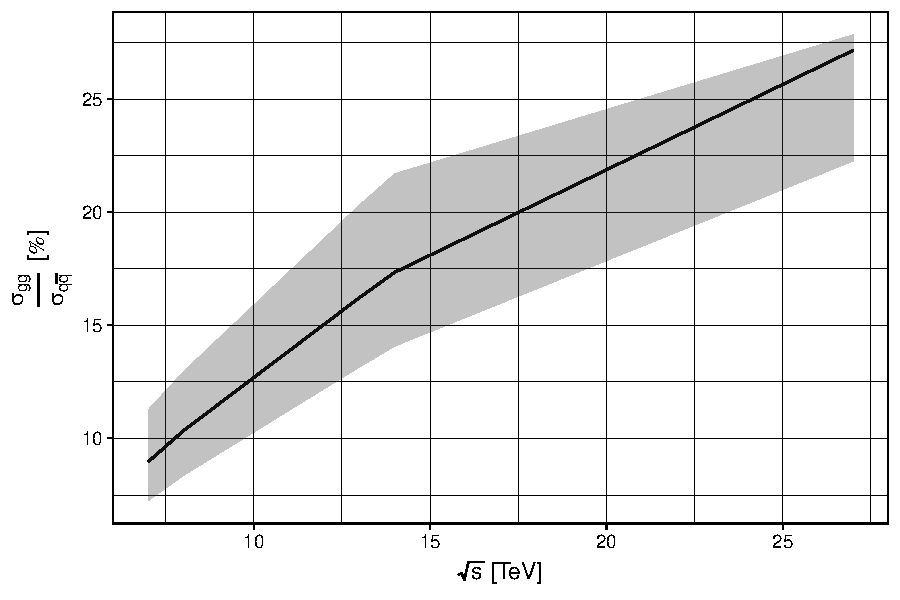
\includegraphics[width=10cm]{./figures/hz_ratio}
		\caption{Examples of Feynman diagrams contributing to $gg \to ZH$ at  LO and
			NLO.}
		\label{fig:hzratio}
	\end{center}
\end{figure}
%%
\par  The leading order (LO) contribution to the $g g \rightarrow Z H$ amplitude, given by one-loop diagrams, was computed exactly in refs.\cite{Kniehl:1990iva, Dicus:1988yh}.However, for the NLO, the virtual corrections contain multi-scale two-loop integrals some of which are still not known analytically ( for the box diagram).  The fiirst computation of the NLO terms has been done by~\cite{Altenkamp:2012sx} using an asymptotic expansion in the limit
$\mt \rightarrow \infty$ and $m_b = 0$, and pointed to a $K$-factor of about $\sim2$.  Later, the computation has been improved via soft gluon resummation, and including NLL terms found in ref.\cite{Harlander:2014wda}, the NLL terms has been matched to the fixed NLO computation of~\cite{Altenkamp:2012sx}.  Top quark mass effects to the  $g g \rightarrow Zh$ process were first implemented using a combination of of large-$\mt$ expansion (LME) and Pad\'e approximants~\cite{Hasselhuhn:2016rqt}. A data-driven approach to extract the gluon fusion dominated non-Drell-Yan part of $Zh$ production using the known relation between  $W H$
and $ Z H$ associated production when only the Drell-Yan component of the two processes is considered has been investigated in ref.\cite{Harlander:2018yns}. The differential distributions of $g g \rightarrow Zh$  at NLO was studied in ref.\cite{Hespel:2015zea} via LO matrix element matching. 
%%
\par More recent studies of the NLO virtual corrections to this process were based on the high-energy~(HE) expansion improved by Pad\'e approximants with the LME, which extended the validity range of the HE expansion \cite{Davies:2020drs}. However, this expansion is only valid for in the invariant mass region $\sqrt{\hat{s}}  \gtrsim 750\, \si{\GeV} $ and $\sqrt{\hat{s}}  \lesssim 350\,  \si{\GeV}$,  which only covers $\sim 32\%$ of the hadronic cross section. Additionally, numerical computation of the 2 loop virtual corrections, though implemented exactly in  \cite{Chen:2020gae}, are rather slow for practical use in MC simulations.  This highlights the importance of an analytical method that can cover the remaining $68\%$ region of the cross-section and can be merged with the HE expansion via Pad\'e approximants. Fortunately, the two-loop corrections to the triangle diagrams can be computed exactly. And the loop integrals appearing in the box correction having no analytic expression can be expanded in small  $Z$ (or Higgs) 
transverse momentum, $\pt$. This method was first used for Higgs pair production in~\cite{Bonciani:2018omm}, to compute the NLO virtual corrections to the box diagrams in the forward kinematics.  In this chapter, I discuss the method and results of the two-loop calculation of the triangle and $\pt$ expansion of $Zh$ process published in~\cite{Alasfar:2021ppe}. 
%%
\par This chapter is structured as follows : In~\autoref{chap6sec:GenNot} contains the general notation for the gluon fusion $Zh$ process . Then, in.. the transverse momentum expansion method is discussed.  Calculation of the LO form-factors in the transverse momentum expansion is shown in... Outline of the two-loop calculation of the triangle topology is illustrated in... Finally, in  I discuss the transverse momentum expansion for the box topology and  .. contains a brief summary and outlook. 

%%%%%%%%%%%%%%%%%%%%%%%%%%%%%%%%%%%%%%%%%%%%%%%%%
\section{General notation \label{chap6sec:GenNot} }
The amplitude  $g^\mu_a(p_1)g^\nu_b(p_2)\to Z^\rho(p_3) h(p_4)$ can be written as
\begin{align}
&&\amp=i \sqrt{2}\frac{\mz \Gfer \as(\mu_R)}{\pi}\delta_{ab}\epsilon^a_\mu(p_1)
\epsilon^b_\nu(p_2)\epsilon_\rho(p_3)\hat{\amp}^{\mu\nu\rho}(p_1,p_2,p_3 ),\\
&&\hat{\amp}^{\mu\nu\rho}(p_1,p_2,p_3 )=\sum_{i=1}^{6}
\mathcal{P}_i^{\mu\nu\rho}(p_1,p_2,p_3 )
\amp_i(\hat{s},\hat{t},\hat{u},\mt,\mh,\mz),
\label{eq:amp}
\end{align}
where  $\mu_R$ is the renormalisation scale and
$\epsilon^a_\mu(p_1)\epsilon^b_\nu(p_2)\epsilon_\rho(p_3)$ are the
polarization vectors of the gluons and the $Z$ boson, respectively.  It is possible to decompose the amplitude into a maximum of $6$ Lorentz structures encapsulated by the 
tensors $\mathcal{P}_i^{\mu\nu\rho}$, we can choose to an orthogonal basis explicitly shown in~\autoref{app:uno}, such that
\begin{equation}
	\mathcal{P}_i^{\mu\nu\rho} \mathcal{P}_j\,_{\mu\nu\rho} = 0, \,\,\, \,\, \text{for}\, i \neq j 
\end{equation}
By this choice one obtains unique form factors corresponding to each projector
\begin{equation}
\amp_i(\hat{s},\hat{t},\hat{u},\mt,\mh,\mz),
\end{equation}
 that are multivariate complex functions of the
top ($\mt$), Higgs ($\mh$) and $Z$ ($\mz$) bosons masses, and of
the partonic Mandelstam variables
\begin{equation}
\hat{s}=(p_1+p_2)^2,~~ \hat{t}=(p_1+p_3)^2,~~ \hat{u}=(p_2+p_3)^2,
\end{equation}
where $\hat{s}+\hat{t}+\hat{u}=\mz^2+\mh^2$ and we took all the momenta to
be incoming. By Bosonic symmetries, the form
The form-factors~ $\amp_i$ can be perturbatively expanded in orders of~$\alpha_s$, 
%%%%%%%
\begin{equation}
\amp_{i} = \sum_{k=0} \left(\frac{\as}{\pi} \right) ^k \amp_i^{(k)}
\label{eq:ampexp}
\end{equation}
Where~$\amp_i^{(0)}$ and $\amp_i^{(1)}$ are the LO and NLO terms, respectively. Using Fermi's Golden Rule, we can write thee Born partonic cross-section as
\begin{equation}
\hat{\sigma}^{(0)}(\hat{s})=
\frac{\mz^2 \Gfer^2 \as(\mu_R)^2}{64 \hat{s}^2(2\pi)^3}
\int^{\hat{t}^+}_{\hat{t}^-}d\hat{t}\sum_i \left|\amp_i^{(0)}\right|^2,
\end{equation}
where
$\hat{t}^\pm=[-\hat{s}+\mh^2+\mz^2\pm\sqrt{(\hat{s}-\mh^2-\mz^2)^2-4\mh^2\mz^2}\,]/2$.
\begin{figure}
	\begin{center}
		\includegraphics[width=12cm]{./figures/Feynman_LO_und_NLO.eps}
		\caption{Examples of Feynman diagrams contributing to $gg \to ZH$ at  LO and
			NLO.}
		\label{fig:dia}
	\end{center}
\end{figure}

The Feynman diagrams that contribute to the $gg \to  ZH$ amplitude up to NLO
can be separated into triangle, box and double-triangle
contributions, the last type appearing for the first time at the
NLO level. Examples of LO (NLO) triangle and box
categories are shown in fig.\ref{fig:dia} $(a)$ - $(c)$
($(d)$ - $(f)$).
Due to the presence of a $\gamma_5$ in the axial coupling of the $Z$ boson to
the fermions in the loop, the projectors $\mathcal{P}_i^{\mu\nu\rho}$ are
proportional to the Levi-Civita total anti-symmetric tensor
$\epsilon^{\alpha\beta\gamma\delta}$ (see appendix \ref{app:uno}),
whose treatment in dimensional regularization is, as well known, delicate
and will be discussed in section \ref{sec:quattro}.

In our calculation we treat all the quarks but the top as massless.
As a consequence, the contribution to the amplitude of the first two generations
vanishes. Concerning the third generation, the contribution of the bottom
is present  in the triangle diagrams with the exchange of a $Z$ boson
(fig.\ref{fig:dia}$(b),(e)$) and in the double-triangle diagrams
(fig.\ref{fig:dia}$(g)$).
A nice observation in ref.\cite{Altenkamp:2012sx} allows to compute
easily the full (top+bottom) triangle contribution. As noticed in that
reference,
the triangle contribution with a $Z$ exchange contains a $ggZ^*$ subamplitude
which in the Landau gauge can be related to the decay of a massive vector boson
with mass $\sqrt{\hat{s}}$ into two massless ones, a process that is
forbidden by
the Landau-Yang theorem \cite{Landau:1948kw,Yang:1950rg}. As a consequence,
the full triangle contribution can be obtained from the top triangle diagrams
with the exchange of the unphysical scalar $G^0$, with the propagator of the
$G^0$ evaluated in the Landau gauge. This part of the top triangle
diagrams  can be obtained from the decay
amplitude of a pseudoscalar boson into two gluons which is  known in
the literature in the full mass dependence up to NLO terms \cite{Spira:1995rr,Aglietti:2006tp}. 

Given the above observation, our calculation of the NLO corrections to
the $gg \to ZH$ amplitude focuses on the analytic evaluation of the
double-triangle (fig.\ref{fig:dia}$(g)$) and two-loop box contributions
(fig.\ref{fig:dia}$(f)$). The former contribution is evaluated exactly.
The latter is evaluated via two different expansions: i) via  a LME, following
ref.\cite{Degrassi:2010eu}, up to and including ${\cal O}(1/\mt^6)$ terms,
which is expected to work below the $2\, \mt$ threshold; ii) via an expansion in
terms of the $Z$ transverse momentum, following ref.\cite{Bonciani:2018omm},
whose details are presented in the next section.

\section{The transverse momentum expansion}
\label{sec:tre}
The transverse momentum of the $Z$  boson can be written in
terms of the Mandelstam variables as
\beq
\pt^2=\frac{\hat{t}\hat{u}-\mz^2\mh^2}{\hat{s}}.
\label{ptdef}
\eeq
From  eq.(\ref{ptdef}), together with the relation between
the Mandelstam variables, one finds 
\beq
\pt^2+\frac{\mh^2+\mz^2}{2}\leq\frac{\hat{s}}{4}+\frac{\dm^2}{\hat{s}},
\label{ptexp}
\eeq
where
$\dm = (\mh^2 -\mz^2)/2$. Eq.(\ref{ptexp}) implies 
$\pt^2/\hat{s} < 1$ that, together with the kinematical constraints
$\mh^2/\hat{s}< 1$ and
$\mz^2/\hat{s} < 1$,  allows the expansion of the amplitude in terms of these
three ratios.


A direct expansion in $\pt$ is not possible at amplitude level, since $\pt$
itself does not appear in the amplitudes. However, as we argued in
ref.\cite{Bonciani:2018omm}, the expansion in $\pt^2/\hat{s}\ll 1$ is equivalent
to an expansion in terms of the ratio of the reduced Mandelstam variables
$t^\prime/s^\prime\ll 1$ or $u^\prime/s^\prime\ll 1$, depending whether we are
considering the process to be in a forward or backward kinematics. The
$s^\prime,\,t^\prime$ and $u^\prime$  variables are defined as
\beq
s^\prime=p_1\cdot p_2=\frac{\hat{s}}{2},~~
t^\prime=p_1\cdot p_3=\frac{\hat{t}-\mz^2}{2},~~ u^\prime =
p_2\cdot p_3=\frac{\hat{u}-\mz^2}{2}
\eeq
and satisfy
\beq
s^\prime + t^\prime + u^\prime =\dm.
\eeq

The cross section of a $2 \to 2$ process can always be expanded into
a forward and backward contribution. Looking at the dependence of $\sigma$
upon $t^\prime,\, u^\prime$ we can write
\bea
\sigma&\propto&\int^{t_f}_{t_i}dt^\prime\mathcal{F}(t^\prime,u^\prime)=
\int^{t_m}_{t_i}dt^\prime\mathcal{F}(t^\prime,u^\prime)+
\int^{t_f}_{t_m}dt^\prime\mathcal{F}(t^\prime,u^\prime) \nn \\
&\sim&\int^{t_m}_{t_i}dt^\prime\mathcal{F}(t^\prime\sim0,u^\prime\sim-s^\prime)+
\int^{t_f}_{t_m}dt^\prime \mathcal{F}(t^\prime\sim -s^\prime,u^\prime\sim0)
\label{eq:forback}
\eea
where $t_i=(\hat{t}^--\mz^2)/2$, $t_f=(\hat{t}^+-\mz^2)/2$ and $t_m$ is the
value of $t^\prime$ at which
$t^\prime =u^\prime=(-s^\prime+\dm)/2$. The two terms in the second
line of eq.(\ref{eq:forback}) represent the expansion in the forward and
backward kinematics, respectively.\\
If the amplitude is symmetric under $t^\prime\leftrightarrow u^\prime$
exchange then
\bea
\sigma&\propto&\int^{t_m}_{t_i}dt^\prime\mathcal{F}(0,-s^\prime)+
\int^{t_f}_{t_m}dt^\prime\mathcal{F}(-s^\prime,0)= \nn \\
&& 
\int^{t_m}_{t_i}dt^\prime\mathcal{F}(0,-s^\prime)+
\int^{t_f}_{t_m}dt^\prime\mathcal{F}(0,-s^\prime)=
\int^{t_f}_{t_i}dt^\prime\mathcal{F}(0,-s^\prime)
\eea
so that the expansion in the forward kinematics actually covers the entire
phase space.

In the case of $gg \to ZH$ the process itself is not symmetric
under the $t^\prime\leftrightarrow u^\prime$ exchange. However, as
can be seen from the explicit expressions of the projectors in appendix
\ref{app:uno},  it can be written as a sum of symmetric and antisymmetric
form factors. To perform only the expansion in the forward kinematics
one can proceed in the following way.
On the symmetric form factors the expansion can be directly performed. 
For the antisymmetric ones,
it is sufficient first  to extract  the overall antisymmetric factor
$(\hat{t}-\hat{u})$  just by multiplying the form factor by $1/(\hat{t}-\hat{u})$,
written as $1/( 2 s^\prime - 4 t^\prime - 2 \dm)$, 
then perform the expansion in the forward
kinematics and finally multiply back by $(\hat{t}-\hat{u})$.

As discussed in ref.\cite{Bonciani:2018omm}, to implement the $\pt$-expansion
at the level of Feynman diagrams it is convenient
to introduce the  vector $r^\mu = p_1^\mu +p_3^\mu$, which satisfies
\beq
r^2= \hat{t},~~ r\cdot p_1=\frac{\hat{t}-\mz^2}{2},~~
r\cdot p_2=-\frac{\hat{t}-\mh^2}{2},
\label{rsp}
\eeq
and therefore can be also written as
\beq
r^\mu =-\frac{\hat{t}-\mh^2}{\hat{s}}p_1^\mu +
\frac{\hat{t}-\mz^2}{\hat{s}} p_2^\mu + r_\perp^\mu =
\frac{t^\prime}{s^\prime}\,(p_2^\mu -p_1^\mu) - \frac{\dm}{s^\prime} \, p_1^\mu +
r_\perp^\mu,
\label{rpp}
\eeq
where
\beq
r_\perp^2=-\pt^2.
\eeq

From eq.(\ref{ptdef}) one obtains
\beq
t^\prime = -\frac{s^\prime}2 \left\{ 1 - \frac{\dm}{s^\prime} \pm
\sqrt{\left( 1 - \frac{\dm}{s^\prime} \right)^2 -
	2 \frac{\pt^2 + \mz^2}{s^\prime}} \right\}
\label{tpdef}
\eeq
that implies  that the expansion in
small $\pt$ (the minus sign case in eq.(\ref{tpdef})) can be realized
at the level of Feynman diagrams, by expanding the propagators
in terms of the vector $r^\mu$ around $r^\mu \sim 0$ or, equivalently,
$p_3^\mu \sim -p_1^\mu$, see eq.(\ref{rpp}). 

The outcome  of the evaluation of the $gg \to ZH$ amplitude via a
$\pt$-expansion is expressed in terms of a series of Master Integrals (MIs)
that are functions of $\hat{s}$ and $\mt^2$ only, and whose coefficients can be
organized in terms of powers of ratios of small  over large parameters
where $\pt^2, \, \mh^2$ and $\mz^2$ are identified as the small parameters while
$\mt^2$ and $\hat{s}$ as the large ones. 
Thus, the range of validity of the expansion depends
on  the condition that $\pt^2$ can be treated as a ``small parameter'' with
respect to $\mt^2$ because all the other ratios, small over
large, are always smaller than 1.

\section{LO Comparison}
\label{sec:Add}
In order to investigate  the range of validity of the evaluation of the
$gg \to ZH$ amplitude via a $\pt$-expansion,  we compare
the exact result for the LO partonic cross
section \cite{Kniehl:1990iva, Dicus:1988yh} with the result obtained
via our $\pt$-expansion. The latter is expressed in terms of the same four MIs
that enter into the analogous calculation of the
$gg \to HH$ LO amplitude \cite{Bonciani:2018omm}, or
\bea
B_0[\hat{s},\mt^2,\mt^2] \equiv  B_0^+, &
B_0[- \hat{s},\mt^2,\mt^2]  \equiv B_0^- , &\\
C_0[0,0,\hat{s},\mt^2,\mt^2,\mt^2]  \equiv  C_0^+  ,& ~~~
C_0[0,0,-\hat{s},\mt^2,\mt^2,\mt^2]  \equiv C_0^- &
\eea
where
\beq
B_0[q^2,m_1^2,m_2^2] = \frac1{i\pi^2}
\int \frac{d^n k}{\mu^{n-4}} \frac1{(k^2 -m_1^2)((k+q)^2-m_2^2)}
\label{Bzero}
\eeq
\begin{align}
%	\specialcell
	{ C_0[q_a^2,q_b^2,(q_a+q_b)^2, m_1^2,m_2^2,m_3^2] = \hfill }\nn  \\
	\frac1{i\pi^2}  \int \frac{d^n k}{\mu^{n-4}} \frac1{[k^2 -m_1^2][(k+q_a)^2-m_2^2]
		[(k-q_b)^2 - m_3^2]} &
	\label{Czero}
\end{align}
are the Passarino-Veltman functions \cite{Passarino:1978jh},
with $n$ the dimension of spacetime and $\mu$ the 't Hooft mass.

As an illustration of our LO result we present the explicit expressions for 
one symmetric, ${\cal A}_2$, and one antisymmetric,
${\cal A}_6$, form factor including the first correction in the ratio of
small over large parameters which will be referred
to as\footnote{With a slight abuse of notation we indicate the
	counting of the orders in the expansion as
	$\mathcal{O}(\pt^{2n})$ that  actually means the inclusion of terms that
	scale   as $(x/y)^n$,   where $x=\pt^2,\, \mz^2,\,\mh^2$ and
	$y=\hat{s},\,\mt^2$, with respect to the $\hat{s}, \mt^2 \to \infty$
	contribution. The latter is indicated as $\mathcal{O}(\pt^0)$ and corresponds
	to the first non zero contribution in the expansion of the diagrams
	in terms of the vector $r^\mu$.} 
${\mathcal O}(\pt^2)$.
We divide the result into triangle ($\triangle$) and
box ($\square$) contribution or
\bea
\mathcal{A}_{2}^{(0, \triangle)} &=& -
\frac{ \pt }{\sqrt{2} \left( \mz^2+\pt^2 \right)} (\hat{s}-\dm)\,
\mt^2 C_0^+,
\label{Adt}\\
\mathcal{A}_{2}^{(0, \square)} &=&
\frac{ \pt }{\sqrt{2} \left(\mz^2+\pt^2 \right)}\, \Biggl\{ \Biggr. \nn \\
&& \Biggl( \mt^2 -\mz^2 \frac{ \hat{s}-6 \mt^2}{4 \hat{s}}-
\pt^2 \frac{ 12 \mt^4-16 \mt^2 \hat{s}+\hat{s}^2}{12 \hat{s}^2}
\Biggr)  B_0^+ \nn \\
&-& \Biggl( \mt^2 -\dm  \frac{\mt^2}{ \left( 4 \mt^2+\hat{s}\right)}
+ \mz^2 \frac{ 24 \mt^4 -6 \mt^2 \hat{s}-
	\hat{s}^2 }{4 \hat{s} \left(4 \mt^2+\hat{s}\right)} -
\nn \\
& & ~~~~~~~\pt^2 \frac{ 48 \mt^6-68 \mt^4 \hat{s}-4
	\mt^2 \hat{s}^2+\hat{s}^3 }{ 12 \hat{s}^2 \left(
	4 \mt^2 +\hat{s} \right) }  \Biggr)
B_0^- \nn \\
&+&\Biggl( 2 \mt^2- \dm +
\mz^2 \frac{3 \mt^2-\hat{s}}{\hat{s} } +
\pt^2  \frac{ 3 \mt^2 \hat{s}-2 \mt^4 }{\hat{s}^2}\Biggr)
\mt^2 \, C_0^- \nn \\
& +&\Biggl( \hat{s}-2 \mt^2 +
\mz^2  \frac{\hat{s}-3 \mt^2 }{\hat{s}}+
\pt^2 \frac{ 2 \mt^4-3 \mt^2 \hat{s}+\hat{s}^2}{\hat{s}^2 }\Biggr)
\mt^2 \, C_0^+ \nn \\
& +&\log \left(\frac{\mt^2}{\mu^2}\right) \frac{ \mt^2}{\left(4
	\mt^2+\hat{s}\right) } \Biggl( \dm + 2  \mz^2
+\pt^2 \frac{2   \hat{s}-2 \mt^2}{3 \hat{s} }\Biggr)\nn  \\
&-&\dm \frac{2 \mt^2}{\left(4 \mt^2+\hat{s}\right) } +
\mz^2  \frac{\hat{s}-12 \mt^2}{4 \left(4 \mt^2+\hat{s}\right)}
+\pt^2 \frac{ 8 \mt^4-2 \mt^2 \hat{s}+ \hat{s}^2 }
{4\hat{s} ( 4\mt^2 + \hat{s})}  \Biggl. \Biggl\},\nn \\
&&
\label{Adb}
\eea
and
\bea
\mathcal{A}_{6}^{(0, \triangle)} &=&  0,
\label{Ast} \\
\mathcal{A}_{6}^{(0, \square)} &= & 
\frac{\hat{t}-\hat{u}}{\hat{s}^2} \,\pt \Biggl[ \frac{\mt^2}2
\Bigl( B_0^- - B_0^+ \Bigr) -\frac{\hat{s}}{4} \nn \\
& -&\frac{2 \mt^2+\hat{s}}{2}\mt^2 \, C_0^- 
+\frac{2 \mt^2-\hat{s}}{2} \mt^2 \,C_0^+  \Biggr],
\label{Asb}
\eea
where in eqs.(\ref{Adb},\ref{Asb}) the $B_0$ functions are understood as the
finite part of the integrals on the right hand side of eq.(\ref{Bzero}).

\begin{figure}[t]
	\centering
	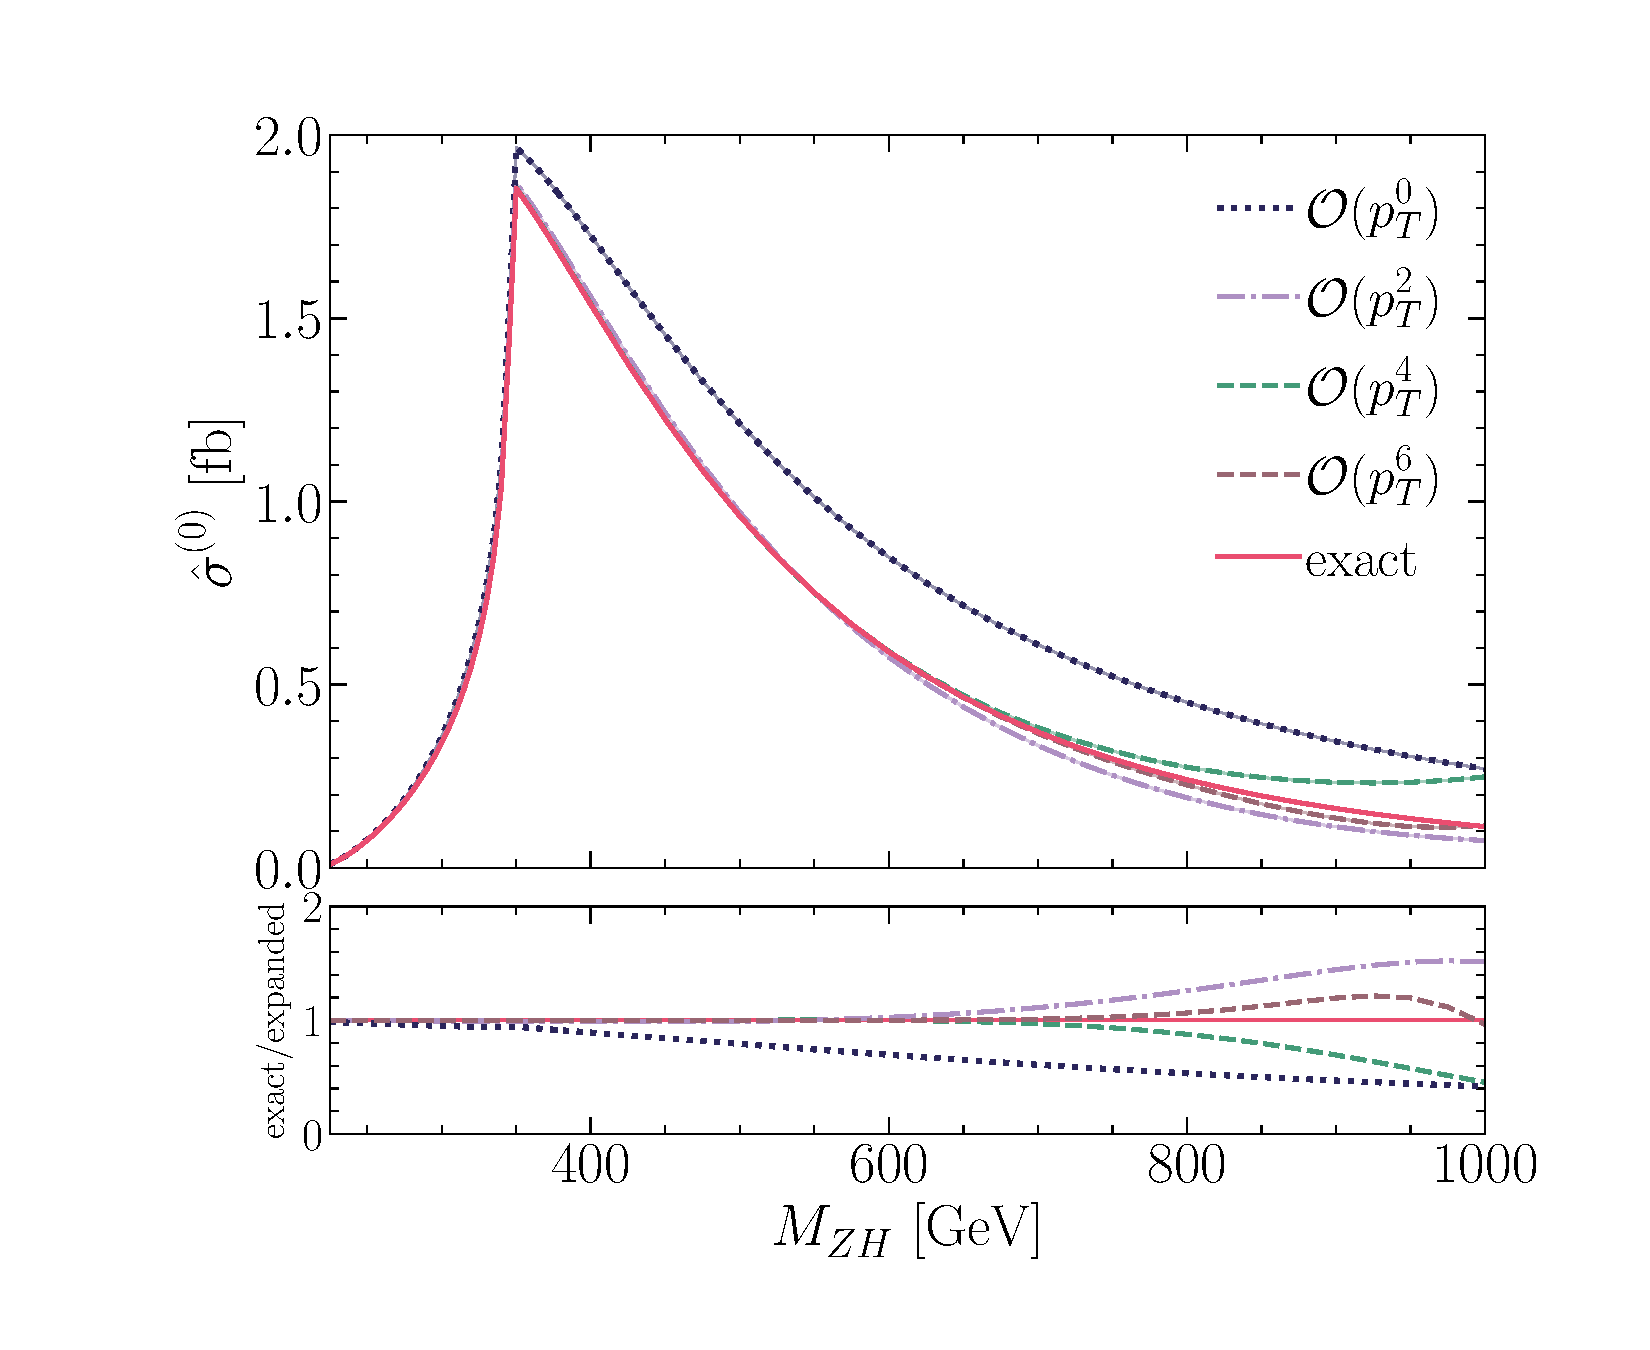
\includegraphics[width=\linewidth]{./figures/LO_ptexp_ratio_1000.pdf}
	\caption{LO partonic cross section
		as a function of the invariant mass $M_{ZH}$.
		The full result (red line) is plotted together with results at
		different orders in the $\pt$-expansion (dashed lines). In the bottom part,
		the ratio of the full result over the $\pt$-expanded one at
		various orders is shown.}
	\label{fig:LO}
\end{figure}

In fig.\ref{fig:LO} the exact partonic LO cross section (red line) is
shown as a function of the invariant mass of the $ZH$ system, $M_{ZH}$, and
compared to various $\pt$-expanded results. 
For the numerical evaluation of the cross section here and in
the following, we used as SM input parameters
\begin{equation}
	\begin{split}
		\mz=91.1876 \,\gev, ~~\mh=125.1 \gev, ~~  \mt=173.21\, \gev, \nn\\
		m_b = 0 \, \gev, ~~G_F= 1.16637\,\gev^{-2},~~ \alpha_s(\mz)=0.118.
	\end{split}
\end{equation}
In the lower part of fig.\ref{fig:LO}  the ratio of the
exact result over the $\pt$-expanded one is shown.  From this ratio
one can see that 
the $\mathcal{O}(\pt^0)$ contribution covers well the $ZH$ invariant mass
region $M_{ZH}\lesssim 2\mt$, corresponding to the range of validity of an
expansion in the large top quark mass. Furthermore, when the contributions up to
$\mathcal{O}(\pt^4)$ are taken into account a remarkable agreement with the
exact result is found up to $M_{ZH}\lesssim 750\gev$.
This agreement is extended to
sligthly higher values of $M_{ZH}$ when the $\mathcal{O}(\pt^6)$ contribution is
included, a finding in close analogy to the result for di-Higgs
production \cite{Bonciani:2018omm}. Similar conclusions can be drawn from table
\ref{tab:partonic}, where it is shown that the partonic cross section
at $\mathcal{O}(\pt^4)$ agrees with the full result for
$M_{ZH} \lesssim 600 \gev$  on the permille level 
and the agreement further improves when $\mathcal{O}(\pt^6)$ terms are included.
As a final remark for this section, we notice that, from the comparison
with the LO exact result, the $\pt$-expanded evaluation of the amplitude is  expected to provide an
accurate result up to $M_{ZH}\sim 700-750\gev$ that corresponds, from
eq.(\ref{ptexp}), to $\pt \lesssim 300-350\, \gev\approx 2\, \mt$.

\begin{table}
	\renewcommand{\arraystretch}{1.2}
	\centering
	\begin{tabular}{| c| c | c | c| c| c|} \hline
		\rowcolor{lightgray}  $M_{ZH}$ [GeV]  & $\mathcal{O}(\pt^0)$ & $\mathcal{O}(\pt^2)$ & $\mathcal{O}(\pt^4)$ & $\mathcal{O}(\pt^6)$ & full \\ \hline 
		\cellcolor{lightgray} 300 & 0.3547 & 0.3393 &  0.3373 &0.3371& 0.3371 \\
		\cellcolor{lightgray} 350 & 1.9385 & 1.8413& 1.8292 &1.8279& 1.8278 \\
		\cellcolor{lightgray} 400 & 1.6990 & 1.5347 & 1.5161 &1.5143& 1.5142 \\
		\cellcolor{lightgray} 600 & 0.8328 & 0.5653 & 0.5804 &0.5792&  0.5794 \\ 
		\cellcolor{lightgray} 750 & 0.5129 & 0.2482 & 0.3129 & 0.2841 &  0.2919 \\ \hline
	\end{tabular}
	\caption{The partonic cross section $\hat{\sigma}^{(0)}$ at
		various orders in $\pt$ and the full computation for several values of $M_{ZH}$. \label{tab:partonic}}
\end{table}

%%%%
\section{ NLO calculation }

Recall that the bare amplitude  reads :

\begin{align}
	-i \mathcal{M} &=  \varepsilon_\mu(p_1) \varepsilon_\nu(p_2)  \,T_R\, \delta_{ab}  \mu_R^{2\epsilon} \as\,  \hat{\mathcal P}_{\mu\nu\rho} \nonumber \\
	& \times S_{\epsilon} \left( \frac{\mu^2_R}{\hat s} \right) ^\epsilon \left[   \mathcal F ^{1 \ell} + \mu_R^{2\epsilon} \as \mu_R^{-2\epsilon} S_{\epsilon} \left( \frac{\mu^2_R}{\hat s} \right) ^\epsilon  \mathcal F ^{2 \ell}  \right]
\end{align}
Where $ \mathcal F^{n\ell}$ is the nth loop form factor, and $\hat{\mathcal P}_{\mu\nu\rho} $ is the normalised projector, written as
\begin{align}
	L^{(1)}_{\mu\nu\rho}  &=  \frac{\hat s}{2} \, \varepsilon_{\mu\nu\rho \xi} \, p_2^\xi -( p_2)_\mu\, \varepsilon_{\nu\rho \xi \lambda } \, p_1^\xi\, p_2 ^\lambda,  \nonumber \\
	L^{(2)}_{\mu\nu\rho}  &= \frac{\hat s}{2} \, \varepsilon_{\mu\nu\rho \xi} \, p_1^\xi -( p_1)_\nu\, \varepsilon_{\mu\rho \xi \lambda } \, p_1^\xi\, p_2 ^\lambda,  \nonumber \\
	\hat{\mathcal P}_{\mu\nu\rho}  &=  \frac{2}{\hat s^3} \left( 	L^{(1)}_{\mu\nu\rho} - 	L^{(2)}_{\mu\nu\rho}\right) .
\end{align}
The 1 loop form factor is given by
\begin{equation}
	\mathcal F ^{1 \ell}  = \frac{m^2}{\hat s} \, C_0(\hat s,0; m,m,m) - \frac{1}{4 \hat s},
\end{equation}
where the last term, not proportional to the mass is corresponding to  the chiral anomaly .
The 2 loop form-factor, can be decomposed in terms of the colour Casimir invariants $ C_A$ and $ C_F$
\begin{equation}
	\mathcal F ^{2 \ell}   = C_F \mathcal F_{CF} ^{2 \ell}  + C_A \mathcal F_{CA} ^{2 \ell}
\end{equation}
The $CA$ part contains double pole $ \mathcal O( 1/\epsilon^2) $  and a single pole $ \mathcal O( 1/\epsilon) $, both  coming from the IR divergence. Whilst the $CF$ part contains a UV divergent pole that needs to be cured via mass renormalisation. The poles do not have a dependence on the renormalisation scale $ \mu_R$, however, there is a dependence on that scale in the finite part.
\subsection{Gluon wavefunction}
We start by the gluon wavefunction renormalisation of the incoming gluons  ( external legs) such that the amplitude is renormalised by $ Z_A^{1/2}$ for each gluon.
\begin{equation}
	Z_A= 1+\as \frac{2}{3\epsilon} \left( \frac{\mu_R^2}{m_t^2} \right) ^\epsilon.
\end{equation}
\subsection{ Strong coupling constant}

The strong couplings constant $ \alpha_s$ renormalisation is done via replacing the bare constant $\alpha_s^0$ with the renormalised one, hence it becomes  $ \alpha^0_s = \frac{\mu_R^{2\epsilon}}{S_\epsilon}  \Zas \alpha_s$, where
\begin{equation}
	\Zas = 1- \frac{\alpha_s}{4 \pi} \, \frac{1}{ \epsilon}\,  \left( \beta_0-\frac{2}{3} \right) \left(\frac{\mu_R^2}{m_t^2} \right) ^\epsilon,
\end{equation}
and the constant $ \beta_0 = \frac{11}{3} C_A -\frac{2}{3}N_f$, where $N_f$ is the number of "active" flavours. In the 5-flavour scheme $N_f=5$.
\subsection{ Top mass}
We use the $\bar{MS}$ scheme for the top mass renormalisation $ m_0 = Z_m m$ , replaced in the propagators, also can be done with multiplying $ \delta Z_m$ with the derivative of the 1 loop form-factor with respect to the  mass., here $Z_m$ is given by
\begin{equation}
	Z_m = 1+ C_F \frac{3}{\epsilon}.
\end{equation}
For the on-shell scheme we add the finite renormalisation term
\begin{equation}
	Z^{OS}_m = 1- 2 C_F
\end{equation}
\subsection{ Larin counter-term}
For the vertex $ -i \bar \psi \gamma_\rho \gamma_5 \psi$, we let $\gamma_5$ naively anti-commute with all $d$-dimensional $\gamma_\mu$'s and then correct that with the finite renormalisation constant
\begin{equation}
	Z_5 = 1- 2\, C_F
\end{equation}

\subsection{All terms together }
The renormalised amplitude is written as
\begin{equation}
	\mathcal M  (\alpha_s, m, \mu_R) = Z_A \mathcal M( \alpha_s^0, m^0).
\end{equation}
Putting all the above substitutions together, we get the renormalised  2 loop form-factor:
\begin{align}
	( \mathcal F ^{2 \ell})^R &= 	\mathcal F ^{2 \ell} -	\mathcal F_{UV} ^{1 \ell}- 	\mathcal F_{UV, m} ^{1 \ell} + \mathcal F_{\text{Larin}} ^{1 \ell}   \\
	\mathcal F_{UV} ^{1 \ell} &= \asr\,\frac{\beta_0}{\epsilon} \left( \frac{\mu_R^2}{\hat s} \right) ^{ -\epsilon}.  \nonumber \\
	\mathcal F_{UV, m} ^{1 \ell} &= \asr \, \left( \frac{3}{\epsilon} -2\right) C_F \left( \frac{\mu_R^2}{\hat s} \right) ^{ -\epsilon} m^0 \partial_m \mathcal F ^{1 \ell} . \nonumber \\
	\\
	\mathcal	F_{\text{Larin}} ^{1 \ell}  &= - \asr \, C_F  \mathcal F ^{1 \ell} .\nonumber
\end{align}
We expand the 1 loop for factor up to order $ \mathcal O(\epsilon) $.
\section{ IR subtraction}
We use the following IR-counter-term
\begin{equation}
	\mathcal F_{IR} ^{1 \ell}  = \frac{e^{\gamma_E \epsilon}}{\Gamma(1-\epsilon)} \, \asr \left( \frac{\beta_0}{\epsilon} + \frac{ C_A}{\epsilon^2} \right)  \, \left(  \frac{\mu_R^2}{\hat s}\right) ^{2\epsilon} \mathcal F ^{1 \ell}
\end{equation}
Here, we expand the 1 loop up to order $ \mathcal O(\epsilon^2) $.
%%%
\section{Outline of the NLO Computation}
\label{sec:quattro}
In this section we discuss our evaluation of the three different types of
diagrams that appear in the virtual corrections to the $gg \to ZH$ amplitude
at the NLO.

The triangle contribution (fig.\ref{fig:dia}$(d),(e)$) was evaluated using the
observation of  ref.\cite{Altenkamp:2012sx}, i.e.~we adapted
the result of ref.\cite{Aglietti:2006tp} for the decay of a
pseudoscalar boson into two gluons  to our case. This contribution is evaluated
exactly and explicit expressions for the form factors are presented in
appendix \ref{app:due}. We notice that if we interpret the exact result
in terms of our counting of the expansion in $\pt$, the $\pt$-expansion of the triangle contribution stops at ${\cal O}(\pt^2)$.

Given the reducible structure of the double-triangle diagrams
(fig.\ref{fig:dia}$(g)$), an exact result for the double-triangle contribution
can be derived in terms of products of one-loop Passarino-Veltman functions
\cite{Passarino:1978jh}.     
Explicit expressions for this contribution are presented in
appendix \ref{app:due}. Although we write the amplitude using a different
tensorial structure with respect to ref.\cite{Davies:2020drs} we checked,
using the relations between the two tensorial structures reported in appendix
\ref{app:uno}, that our result is in agreement with the one presented
in ref.\cite{Hasselhuhn:2016rqt}.

The box contribution (fig.\ref{fig:dia}$(f)$) was computed evaluating
the two-loop multi-scale Feynman integrals via two different expansions:
a LME up to and including $\mathcal{O}(1/\mt^6)$ terms, and  an
expansion in the transverse momentum up to and including
${\cal O}(\pt^4)$ terms.
The former expansion was used as ``control'' expansion of the latter.
Indeed, the $\pt$-expanded result actually ``contains'' the LME one. The LME
differs from the expansion in $\pt$ by the fact that $\hat{s}$ is
treated as a small parameter with respect to $\mt^2$, and not on the same
footing as in the latter case. This implies that if the $\pt$-expanded result is
further expanded in terms of the  $\hat{s}/\mt^2$ ratio the LME result has to
be recovered. This way, we were able to reproduce, at the analytic level,
our LME result. 


We conclude this section outlining some technical details concerning our
computation.  We generated the amplitudes using \texttt{FeynArts} \cite{Hahn:2000kx} and
contracted them with the projectors as defined in appendix \ref{app:uno}
using \texttt{FeynCalc }\cite{Mertig:1990an,Shtabovenko:2016sxi} and in-house
Mathematica routines.  We used  dimensional regularization and
the rule for the contraction of two epsilon tensors written in terms of
the determinant of $n$-dimensional metric tensors. This is not a consistent
procedure and  needs to be corrected. A correction term should be added
\cite{Larin:1993tq} to the form factors computed as described
above, $\amp^{(1,ndr)}_i$, namely
\beq
\amp^{(1)}_i = \amp^{(1,ndr)}_i -\frac{\as}{\pi} C_F \amp_i^{(0)}~.
\label{eq:larin}
\eeq
In order to check eq.(\ref{eq:larin}), following ref.\cite{Degrassi:2011vq}
we bypassed the problem of the treatment of 
$\gamma_5$ in dimensional regularization computing the amplitude via
a LME working in 4 dimension, employing the Background Field Method (BFM)
\cite{Abbott:1980hw} and using as regularization scheme  the Pauli-Villars
method. This result was compared with the LME evaluation of
$\amp^{(1,ndr)}_i$, finding that the difference between the two
evaluations was indeed given by the second term on the right-hand-side of
eq.(\ref{eq:larin}).

After the contraction of the epsilon tensors the diagrams were expanded as
described in section \ref{sec:tre}. They were reduced to MIs
using \texttt{FIRE} \cite{Smirnov:2014hma} and \texttt{LiteRed} \cite{Lee:2013mka}. The
resulting MIs were exactly the same as previously found for di-Higgs
production \cite{Bonciani:2018omm}. Nearly all of them are expressed
in terms of generalised harmonic polylogarithms with the exception of
two elliptic integrals \cite{vonManteuffel:2017hms, Bonciani:2018uvv}.
The top quark mass was renormalized in the onshell scheme\footnote{Different choices
	for the renormalized top mass can be easily implemented in our calculation.}
and the IR poles were subtracted as in ref.\cite{Degrassi:2016vss}.

\section{Conclusion \label{sec:conclusion}}
In this paper, we computed  the two-loop NLO virtual corrections to the 
$gg \to ZH$ process. Among the two-loop Feynman diagrams contributing
to the process,  the ones belonging to the triangle and
double-triangle topology were computed exactly. The ones  belonging 
to the box topology, which contain multiscale integrals, were evaluated via an
expansion in the $Z$ transverse momentum. This novel approach of
computing a process in the forward kinematics
was originally proposed in ref.\cite{Bonciani:2018omm} for
double Higgs production where the particles in the final state have
the same mass. In this paper,  we  extended
the method to the more general case of two different masses in the
final state and to a process whose amplitude is not symmetric
under the  $\hat{t}\leftrightarrow \hat{u}$ exchange.

The result of the evaluation of the box contribution is expressed,
both at one- and two-loop level, in terms of the
same set of MIs that was found in ref.\cite{Bonciani:2018omm} for
double Higgs production.  The two-loop MIs  can be all
expressed in terms of generalised harmonic polylogarithms with the
exception of two elliptic integrals.

As we have shown explicitly at the LO, the range of validity of our
computation covers values of the invariant mass
$M_{ZH}\lesssim 750\text{ GeV}$ corresponding to 98.5\% of the phase
space at LHC energies.  We showed that few terms in our
expansion were sufficient to obtain an incredible good agreement with the
numerical evalution of ${\mathcal V}_{fin}$ presented in ref.\cite{Chen:2020gae},
at the level of a permille or less difference between our analytic result and the numerical one.

The advantage of our analytic approach compared to the numerical
calculation is also in the computing time. With an average evaluation
time of half a second per phase space point, an inclusion into a Monte Carlo
programme is realistic. Due to the flexibility of our analytic
results, an application to beyond-the-Standard Model is certainly
possible.

Finally, we remark that our calculation complements
nicely the results obtained in ref.\cite{Davies:2020drs} using a high-energy
expansion, that according to the authors provides precise results for
$\pt \gtrsim 200\gev$. The merging of the two analyses is going to provide
a result that covers the whole phase space, can be easily implemented into a
Monte Carlo code and  presents the flexibility of an analytic calculation.